\documentclass{article} % For LaTeX2e
\usepackage{iclr2019,times}

\usepackage{amssymb}

\usepackage{hyperref}
\usepackage{url}
\usepackage{bm}
\usepackage{graphicx,array} \graphicspath{{figures/}}
\usepackage{amsmath}
\usepackage{color}

% % Optional math commands from https://github.com/goodfeli/dlbook_notation.
% %%%%% NEW MATH DEFINITIONS %%%%%

\usepackage{amsmath,amsfonts,bm}

% Mark sections of captions for referring to divisions of figures
\newcommand{\figleft}{{\em (Left)}}
\newcommand{\figcenter}{{\em (Center)}}
\newcommand{\figright}{{\em (Right)}}
\newcommand{\figtop}{{\em (Top)}}
\newcommand{\figbottom}{{\em (Bottom)}}
\newcommand{\captiona}{{\em (a)}}
\newcommand{\captionb}{{\em (b)}}
\newcommand{\captionc}{{\em (c)}}
\newcommand{\captiond}{{\em (d)}}

% Highlight a newly defined term
\newcommand{\newterm}[1]{{\bf #1}}


% Figure reference, lower-case.
\def\figref#1{figure~\ref{#1}}
% Figure reference, capital. For start of sentence
\def\Figref#1{Figure~\ref{#1}}
\def\twofigref#1#2{figures \ref{#1} and \ref{#2}}
\def\quadfigref#1#2#3#4{figures \ref{#1}, \ref{#2}, \ref{#3} and \ref{#4}}
% Section reference, lower-case.
\def\secref#1{section~\ref{#1}}
% Section reference, capital.
\def\Secref#1{Section~\ref{#1}}
% Reference to two sections.
\def\twosecrefs#1#2{sections \ref{#1} and \ref{#2}}
% Reference to three sections.
\def\secrefs#1#2#3{sections \ref{#1}, \ref{#2} and \ref{#3}}
% Reference to an equation, lower-case.
\def\eqref#1{equation~\ref{#1}}
% Reference to an equation, upper case
\def\Eqref#1{Equation~\ref{#1}}
% A raw reference to an equation---avoid using if possible
\def\plaineqref#1{\ref{#1}}
% Reference to a chapter, lower-case.
\def\chapref#1{chapter~\ref{#1}}
% Reference to an equation, upper case.
\def\Chapref#1{Chapter~\ref{#1}}
% Reference to a range of chapters
\def\rangechapref#1#2{chapters\ref{#1}--\ref{#2}}
% Reference to an algorithm, lower-case.
\def\algref#1{algorithm~\ref{#1}}
% Reference to an algorithm, upper case.
\def\Algref#1{Algorithm~\ref{#1}}
\def\twoalgref#1#2{algorithms \ref{#1} and \ref{#2}}
\def\Twoalgref#1#2{Algorithms \ref{#1} and \ref{#2}}
% Reference to a part, lower case
\def\partref#1{part~\ref{#1}}
% Reference to a part, upper case
\def\Partref#1{Part~\ref{#1}}
\def\twopartref#1#2{parts \ref{#1} and \ref{#2}}

\def\ceil#1{\lceil #1 \rceil}
\def\floor#1{\lfloor #1 \rfloor}
\def\1{\bm{1}}
\newcommand{\train}{\mathcal{D}}
\newcommand{\valid}{\mathcal{D_{\mathrm{valid}}}}
\newcommand{\test}{\mathcal{D_{\mathrm{test}}}}

\def\eps{{\epsilon}}


% Random variables
\def\reta{{\textnormal{$\eta$}}}
\def\ra{{\textnormal{a}}}
\def\rb{{\textnormal{b}}}
\def\rc{{\textnormal{c}}}
\def\rd{{\textnormal{d}}}
\def\re{{\textnormal{e}}}
\def\rf{{\textnormal{f}}}
\def\rg{{\textnormal{g}}}
\def\rh{{\textnormal{h}}}
\def\ri{{\textnormal{i}}}
\def\rj{{\textnormal{j}}}
\def\rk{{\textnormal{k}}}
\def\rl{{\textnormal{l}}}
% rm is already a command, just don't name any random variables m
\def\rn{{\textnormal{n}}}
\def\ro{{\textnormal{o}}}
\def\rp{{\textnormal{p}}}
\def\rq{{\textnormal{q}}}
\def\rr{{\textnormal{r}}}
\def\rs{{\textnormal{s}}}
\def\rt{{\textnormal{t}}}
\def\ru{{\textnormal{u}}}
\def\rv{{\textnormal{v}}}
\def\rw{{\textnormal{w}}}
\def\rx{{\textnormal{x}}}
\def\ry{{\textnormal{y}}}
\def\rz{{\textnormal{z}}}

% Random vectors
\def\rvepsilon{{\mathbf{\epsilon}}}
\def\rvtheta{{\mathbf{\theta}}}
\def\rva{{\mathbf{a}}}
\def\rvb{{\mathbf{b}}}
\def\rvc{{\mathbf{c}}}
\def\rvd{{\mathbf{d}}}
\def\rve{{\mathbf{e}}}
\def\rvf{{\mathbf{f}}}
\def\rvg{{\mathbf{g}}}
\def\rvh{{\mathbf{h}}}
\def\rvu{{\mathbf{i}}}
\def\rvj{{\mathbf{j}}}
\def\rvk{{\mathbf{k}}}
\def\rvl{{\mathbf{l}}}
\def\rvm{{\mathbf{m}}}
\def\rvn{{\mathbf{n}}}
\def\rvo{{\mathbf{o}}}
\def\rvp{{\mathbf{p}}}
\def\rvq{{\mathbf{q}}}
\def\rvr{{\mathbf{r}}}
\def\rvs{{\mathbf{s}}}
\def\rvt{{\mathbf{t}}}
\def\rvu{{\mathbf{u}}}
\def\rvv{{\mathbf{v}}}
\def\rvw{{\mathbf{w}}}
\def\rvx{{\mathbf{x}}}
\def\rvy{{\mathbf{y}}}
\def\rvz{{\mathbf{z}}}

% Elements of random vectors
\def\erva{{\textnormal{a}}}
\def\ervb{{\textnormal{b}}}
\def\ervc{{\textnormal{c}}}
\def\ervd{{\textnormal{d}}}
\def\erve{{\textnormal{e}}}
\def\ervf{{\textnormal{f}}}
\def\ervg{{\textnormal{g}}}
\def\ervh{{\textnormal{h}}}
\def\ervi{{\textnormal{i}}}
\def\ervj{{\textnormal{j}}}
\def\ervk{{\textnormal{k}}}
\def\ervl{{\textnormal{l}}}
\def\ervm{{\textnormal{m}}}
\def\ervn{{\textnormal{n}}}
\def\ervo{{\textnormal{o}}}
\def\ervp{{\textnormal{p}}}
\def\ervq{{\textnormal{q}}}
\def\ervr{{\textnormal{r}}}
\def\ervs{{\textnormal{s}}}
\def\ervt{{\textnormal{t}}}
\def\ervu{{\textnormal{u}}}
\def\ervv{{\textnormal{v}}}
\def\ervw{{\textnormal{w}}}
\def\ervx{{\textnormal{x}}}
\def\ervy{{\textnormal{y}}}
\def\ervz{{\textnormal{z}}}

% Random matrices
\def\rmA{{\mathbf{A}}}
\def\rmB{{\mathbf{B}}}
\def\rmC{{\mathbf{C}}}
\def\rmD{{\mathbf{D}}}
\def\rmE{{\mathbf{E}}}
\def\rmF{{\mathbf{F}}}
\def\rmG{{\mathbf{G}}}
\def\rmH{{\mathbf{H}}}
\def\rmI{{\mathbf{I}}}
\def\rmJ{{\mathbf{J}}}
\def\rmK{{\mathbf{K}}}
\def\rmL{{\mathbf{L}}}
\def\rmM{{\mathbf{M}}}
\def\rmN{{\mathbf{N}}}
\def\rmO{{\mathbf{O}}}
\def\rmP{{\mathbf{P}}}
\def\rmQ{{\mathbf{Q}}}
\def\rmR{{\mathbf{R}}}
\def\rmS{{\mathbf{S}}}
\def\rmT{{\mathbf{T}}}
\def\rmU{{\mathbf{U}}}
\def\rmV{{\mathbf{V}}}
\def\rmW{{\mathbf{W}}}
\def\rmX{{\mathbf{X}}}
\def\rmY{{\mathbf{Y}}}
\def\rmZ{{\mathbf{Z}}}

% Elements of random matrices
\def\ermA{{\textnormal{A}}}
\def\ermB{{\textnormal{B}}}
\def\ermC{{\textnormal{C}}}
\def\ermD{{\textnormal{D}}}
\def\ermE{{\textnormal{E}}}
\def\ermF{{\textnormal{F}}}
\def\ermG{{\textnormal{G}}}
\def\ermH{{\textnormal{H}}}
\def\ermI{{\textnormal{I}}}
\def\ermJ{{\textnormal{J}}}
\def\ermK{{\textnormal{K}}}
\def\ermL{{\textnormal{L}}}
\def\ermM{{\textnormal{M}}}
\def\ermN{{\textnormal{N}}}
\def\ermO{{\textnormal{O}}}
\def\ermP{{\textnormal{P}}}
\def\ermQ{{\textnormal{Q}}}
\def\ermR{{\textnormal{R}}}
\def\ermS{{\textnormal{S}}}
\def\ermT{{\textnormal{T}}}
\def\ermU{{\textnormal{U}}}
\def\ermV{{\textnormal{V}}}
\def\ermW{{\textnormal{W}}}
\def\ermX{{\textnormal{X}}}
\def\ermY{{\textnormal{Y}}}
\def\ermZ{{\textnormal{Z}}}

% Vectors
\def\vzero{{\bm{0}}}
\def\vone{{\bm{1}}}
\def\vmu{{\bm{\mu}}}
\def\vtheta{{\bm{\theta}}}
\def\va{{\bm{a}}}
\def\vb{{\bm{b}}}
\def\vc{{\bm{c}}}
\def\vd{{\bm{d}}}
\def\ve{{\bm{e}}}
\def\vf{{\bm{f}}}
\def\vg{{\bm{g}}}
\def\vh{{\bm{h}}}
\def\vi{{\bm{i}}}
\def\vj{{\bm{j}}}
\def\vk{{\bm{k}}}
\def\vl{{\bm{l}}}
\def\vm{{\bm{m}}}
\def\vn{{\bm{n}}}
\def\vo{{\bm{o}}}
\def\vp{{\bm{p}}}
\def\vq{{\bm{q}}}
\def\vr{{\bm{r}}}
\def\vs{{\bm{s}}}
\def\vt{{\bm{t}}}
\def\vu{{\bm{u}}}
\def\vv{{\bm{v}}}
\def\vw{{\bm{w}}}
\def\vx{{\bm{x}}}
\def\vy{{\bm{y}}}
\def\vz{{\bm{z}}}

% Elements of vectors
\def\evalpha{{\alpha}}
\def\evbeta{{\beta}}
\def\evepsilon{{\epsilon}}
\def\evlambda{{\lambda}}
\def\evomega{{\omega}}
\def\evmu{{\mu}}
\def\evpsi{{\psi}}
\def\evsigma{{\sigma}}
\def\evtheta{{\theta}}
\def\eva{{a}}
\def\evb{{b}}
\def\evc{{c}}
\def\evd{{d}}
\def\eve{{e}}
\def\evf{{f}}
\def\evg{{g}}
\def\evh{{h}}
\def\evi{{i}}
\def\evj{{j}}
\def\evk{{k}}
\def\evl{{l}}
\def\evm{{m}}
\def\evn{{n}}
\def\evo{{o}}
\def\evp{{p}}
\def\evq{{q}}
\def\evr{{r}}
\def\evs{{s}}
\def\evt{{t}}
\def\evu{{u}}
\def\evv{{v}}
\def\evw{{w}}
\def\evx{{x}}
\def\evy{{y}}
\def\evz{{z}}

% Matrix
\def\mA{{\bm{A}}}
\def\mB{{\bm{B}}}
\def\mC{{\bm{C}}}
\def\mD{{\bm{D}}}
\def\mE{{\bm{E}}}
\def\mF{{\bm{F}}}
\def\mG{{\bm{G}}}
\def\mH{{\bm{H}}}
\def\mI{{\bm{I}}}
\def\mJ{{\bm{J}}}
\def\mK{{\bm{K}}}
\def\mL{{\bm{L}}}
\def\mM{{\bm{M}}}
\def\mN{{\bm{N}}}
\def\mO{{\bm{O}}}
\def\mP{{\bm{P}}}
\def\mQ{{\bm{Q}}}
\def\mR{{\bm{R}}}
\def\mS{{\bm{S}}}
\def\mT{{\bm{T}}}
\def\mU{{\bm{U}}}
\def\mV{{\bm{V}}}
\def\mW{{\bm{W}}}
\def\mX{{\bm{X}}}
\def\mY{{\bm{Y}}}
\def\mZ{{\bm{Z}}}
\def\mBeta{{\bm{\beta}}}
\def\mPhi{{\bm{\Phi}}}
\def\mLambda{{\bm{\Lambda}}}
\def\mSigma{{\bm{\Sigma}}}

% Tensor
\DeclareMathAlphabet{\mathsfit}{\encodingdefault}{\sfdefault}{m}{sl}
\SetMathAlphabet{\mathsfit}{bold}{\encodingdefault}{\sfdefault}{bx}{n}
\newcommand{\tens}[1]{\bm{\mathsfit{#1}}}
\def\tA{{\tens{A}}}
\def\tB{{\tens{B}}}
\def\tC{{\tens{C}}}
\def\tD{{\tens{D}}}
\def\tE{{\tens{E}}}
\def\tF{{\tens{F}}}
\def\tG{{\tens{G}}}
\def\tH{{\tens{H}}}
\def\tI{{\tens{I}}}
\def\tJ{{\tens{J}}}
\def\tK{{\tens{K}}}
\def\tL{{\tens{L}}}
\def\tM{{\tens{M}}}
\def\tN{{\tens{N}}}
\def\tO{{\tens{O}}}
\def\tP{{\tens{P}}}
\def\tQ{{\tens{Q}}}
\def\tR{{\tens{R}}}
\def\tS{{\tens{S}}}
\def\tT{{\tens{T}}}
\def\tU{{\tens{U}}}
\def\tV{{\tens{V}}}
\def\tW{{\tens{W}}}
\def\tX{{\tens{X}}}
\def\tY{{\tens{Y}}}
\def\tZ{{\tens{Z}}}


% Graph
\def\gA{{\mathcal{A}}}
\def\gB{{\mathcal{B}}}
\def\gC{{\mathcal{C}}}
\def\gD{{\mathcal{D}}}
\def\gE{{\mathcal{E}}}
\def\gF{{\mathcal{F}}}
\def\gG{{\mathcal{G}}}
\def\gH{{\mathcal{H}}}
\def\gI{{\mathcal{I}}}
\def\gJ{{\mathcal{J}}}
\def\gK{{\mathcal{K}}}
\def\gL{{\mathcal{L}}}
\def\gM{{\mathcal{M}}}
\def\gN{{\mathcal{N}}}
\def\gO{{\mathcal{O}}}
\def\gP{{\mathcal{P}}}
\def\gQ{{\mathcal{Q}}}
\def\gR{{\mathcal{R}}}
\def\gS{{\mathcal{S}}}
\def\gT{{\mathcal{T}}}
\def\gU{{\mathcal{U}}}
\def\gV{{\mathcal{V}}}
\def\gW{{\mathcal{W}}}
\def\gX{{\mathcal{X}}}
\def\gY{{\mathcal{Y}}}
\def\gZ{{\mathcal{Z}}}

% Sets
\def\sA{{\mathbb{A}}}
\def\sB{{\mathbb{B}}}
\def\sC{{\mathbb{C}}}
\def\sD{{\mathbb{D}}}
% Don't use a set called E, because this would be the same as our symbol
% for expectation.
\def\sF{{\mathbb{F}}}
\def\sG{{\mathbb{G}}}
\def\sH{{\mathbb{H}}}
\def\sI{{\mathbb{I}}}
\def\sJ{{\mathbb{J}}}
\def\sK{{\mathbb{K}}}
\def\sL{{\mathbb{L}}}
\def\sM{{\mathbb{M}}}
\def\sN{{\mathbb{N}}}
\def\sO{{\mathbb{O}}}
\def\sP{{\mathbb{P}}}
\def\sQ{{\mathbb{Q}}}
\def\sR{{\mathbb{R}}}
\def\sS{{\mathbb{S}}}
\def\sT{{\mathbb{T}}}
\def\sU{{\mathbb{U}}}
\def\sV{{\mathbb{V}}}
\def\sW{{\mathbb{W}}}
\def\sX{{\mathbb{X}}}
\def\sY{{\mathbb{Y}}}
\def\sZ{{\mathbb{Z}}}

% Entries of a matrix
\def\emLambda{{\Lambda}}
\def\emA{{A}}
\def\emB{{B}}
\def\emC{{C}}
\def\emD{{D}}
\def\emE{{E}}
\def\emF{{F}}
\def\emG{{G}}
\def\emH{{H}}
\def\emI{{I}}
\def\emJ{{J}}
\def\emK{{K}}
\def\emL{{L}}
\def\emM{{M}}
\def\emN{{N}}
\def\emO{{O}}
\def\emP{{P}}
\def\emQ{{Q}}
\def\emR{{R}}
\def\emS{{S}}
\def\emT{{T}}
\def\emU{{U}}
\def\emV{{V}}
\def\emW{{W}}
\def\emX{{X}}
\def\emY{{Y}}
\def\emZ{{Z}}
\def\emSigma{{\Sigma}}

% entries of a tensor
% Same font as tensor, without \bm wrapper
\newcommand{\etens}[1]{\mathsfit{#1}}
\def\etLambda{{\etens{\Lambda}}}
\def\etA{{\etens{A}}}
\def\etB{{\etens{B}}}
\def\etC{{\etens{C}}}
\def\etD{{\etens{D}}}
\def\etE{{\etens{E}}}
\def\etF{{\etens{F}}}
\def\etG{{\etens{G}}}
\def\etH{{\etens{H}}}
\def\etI{{\etens{I}}}
\def\etJ{{\etens{J}}}
\def\etK{{\etens{K}}}
\def\etL{{\etens{L}}}
\def\etM{{\etens{M}}}
\def\etN{{\etens{N}}}
\def\etO{{\etens{O}}}
\def\etP{{\etens{P}}}
\def\etQ{{\etens{Q}}}
\def\etR{{\etens{R}}}
\def\etS{{\etens{S}}}
\def\etT{{\etens{T}}}
\def\etU{{\etens{U}}}
\def\etV{{\etens{V}}}
\def\etW{{\etens{W}}}
\def\etX{{\etens{X}}}
\def\etY{{\etens{Y}}}
\def\etZ{{\etens{Z}}}

% The true underlying data generating distribution
\newcommand{\pdata}{p_{\rm{data}}}
% The empirical distribution defined by the training set
\newcommand{\ptrain}{\hat{p}_{\rm{data}}}
\newcommand{\Ptrain}{\hat{P}_{\rm{data}}}
% The model distribution
\newcommand{\pmodel}{p_{\rm{model}}}
\newcommand{\Pmodel}{P_{\rm{model}}}
\newcommand{\ptildemodel}{\tilde{p}_{\rm{model}}}
% Stochastic autoencoder distributions
\newcommand{\pencode}{p_{\rm{encoder}}}
\newcommand{\pdecode}{p_{\rm{decoder}}}
\newcommand{\precons}{p_{\rm{reconstruct}}}

\newcommand{\laplace}{\mathrm{Laplace}} % Laplace distribution

\newcommand{\E}{\mathbb{E}}
\newcommand{\Ls}{\mathcal{L}}
\newcommand{\R}{\mathbb{R}}
\newcommand{\emp}{\tilde{p}}
\newcommand{\lr}{\alpha}
\newcommand{\reg}{\lambda}
\newcommand{\rect}{\mathrm{rectifier}}
\newcommand{\softmax}{\mathrm{softmax}}
\newcommand{\sigmoid}{\sigma}
\newcommand{\softplus}{\zeta}
\newcommand{\KL}{D_{\mathrm{KL}}}
\newcommand{\Var}{\mathrm{Var}}
\newcommand{\standarderror}{\mathrm{SE}}
\newcommand{\Cov}{\mathrm{Cov}}
% Wolfram Mathworld says $L^2$ is for function spaces and $\ell^2$ is for vectors
% But then they seem to use $L^2$ for vectors throughout the site, and so does
% wikipedia.
\newcommand{\normlzero}{L^0}
\newcommand{\normlone}{L^1}
\newcommand{\normltwo}{L^2}
\newcommand{\normlp}{L^p}
\newcommand{\normmax}{L^\infty}

\newcommand{\parents}{Pa} % See usage in notation.tex. Chosen to match Daphne's book.

\DeclareMathOperator*{\argmax}{arg\,max}
\DeclareMathOperator*{\argmin}{arg\,min}

\DeclareMathOperator{\sign}{sign}
\DeclareMathOperator{\Tr}{Tr}
\let\ab\allowbreak





\newcommand{\figref}[1]{Figure~\ref{fig:#1}}
\newcommand{\tabref}[1]{Table~\ref{tab:#1}}
\newcommand{\secref}[1]{Section~\ref{sec:#1}}
%\newcommand{\secref}[1]{\S\ref{sec:#1}}
\newcommand{\eqnref}[1]{(\ref{eqn:#1})}

\renewcommand{\b}[1]{{\bm{#1}}}   % bold symbol

% MATH SYMBOLS
\newcommand{\1}{\b{1}}              % all-ones vector
\newcommand{\0}{\b{0}}              % all-zero vector
\newcommand{\g}[1]{\b{#1}}
\newcommand{\G}{\mathcal{G}}
\newcommand{\V}{\mathcal{V}}
\newcommand{\E}{\mathcal{E}}
\newcommand{\C}{\mathcal{C}}
\newcommand{\B}{\mathcal{B}}
\renewcommand{\L}{\b{L}}
\newcommand{\tL}{\tilde{\L}}
\newcommand{\W}{\b{W}}
\newcommand{\I}{\b{I}}
\newcommand{\D}{\b{D}}
\newcommand{\U}{\b{U}}
\newcommand{\x}{\b{x}}
\newcommand{\X}{\b{X}}
\newcommand{\y}{\b{y}}
\newcommand{\Y}{\b{Y}}
\newcommand{\bu}{\b{u}}
\newcommand{\f}{\b{f}}
\newcommand{\trans}{^\intercal}
\newcommand{\R}{\mathbb{R}}
\newcommand{\bLambda}{\b{\Lambda}}
\newcommand{\blambda}{\b{\lambda}}
\newcommand{\bO}{\mathcal{O}}
\newcommand{\T}{\mathcal{T}}
\DeclareMathOperator*{\esp}{E}
\DeclareMathOperator*{\var}{Var}
\DeclareMathOperator*{\vect}{vec}
\DeclareMathOperator*{\argmin}{arg \, min}

\title{DeepSphere}
% Keywords: equivariance, spherical CNN, graph NN
%\title{DeepSphere: an equivariant spherical CNN based on a graph NN}
% Exploiting symmetries with Graph Neural Networks
% Another reason to use Graph Neural Networks: exploiting symmetries
% Another case for Graph Neural Networks: exploiting symmetries
% The case for using graphs to reason / compute / solve continuous problems.

\author{Michaël Defferrard \\
Institute of Electrical Engineering \\
EPFL, Lausanne, Switzerland \\
\texttt{michaël.defferrard@epfl.ch} \\
\And
Nathanaël Perraudin \\
Swiss Data Science Center (SDSC) \\
Zurich, Switzerland \\
\texttt{nathanael.perraudin@sdsc.ethz.ch} \\
}

\newcommand{\fix}{\marginpar{FIX}}
\newcommand{\new}{\marginpar{NEW}}
\newcommand{\todo}[1]{{\color[rgb]{.6,.1,.6}{#1}}}
\newcommand{\nati}[1]{{\color[rgb]{.1,.6,.1}{#1}}}

%\iclrfinalcopy % Uncomment for camera-ready version, but NOT for submission.
\begin{document}

\maketitle

\begin{abstract}
	\todo{TODO:
		\begin{enumerate}
			\item add figures from DeepSphere cosmo
			\item reorganize thoughts
			\item fill the holes
			\item coherent and consistent story
		\end{enumerate}
	}
\end{abstract}

\section{Introduction}

There has been a lot of interest recently [xx] in studying and developing NN architectures that exploit symmetries in the data by being equivariant (or invariant) to a select group of symmetric transformations (symmetry group).
In this paper, we argue that graph neural networks are a flexible model (albeit not the most general) to exploit such symmetries.
graphs are a great support for computations on many domains.

%\section{Related Work}
\todo{Related work as a paragraph. Mention interest in spherical CNNs for various applications, importance of equivariance and invariance, previous exploratory work from Renata and ourselves.}

As there is no equivalent to the uniform sampling of Euclidean space on the sphere, sphere pixelizations have been engineered to have some characteristics: equirectangular (a.k.a. equiangular or geographic) is simple\footnote{It is used in most spherical CNNs cite Cohen, renata, esteves}. HEALPix is equal-area\footnote{That is important for white noise to stay white.}, hierarchical, and has a fast SHT \citep{healpix}, GLESP features an exact (to machine precision) SHT \citep{glesp}, sympix?, cubed-sphere?.
\todo{look at the wording in sympix}
\todo{maybe have a table, or a list of desired properties from a sampling}

\todo{What is the problem we want to solve? Identify it. Our solution: allow any sampling, flexibility.}
\todo{there is a compromise about the sampling quality (how far from uniform) and how close discrete computations can be made to the true continuous ones}
masked data is a pain for ML in general (with graphs, we can just make it disappear)

\todo{Most of our view is shaped by cosmo. What is going on in other fields (climate, weather)? Do they have their own samplings? Cosmo seems the most advanced for SP on the sphere.}

\todo{We can take here a different stance than: "we'll use whatever method gives the best performance". SHTs are the standard analysis tool on the sphere. People not only want to apply learned filters, but designed ones (e.g., Gaussian smoothing), people want to interpret and see the spectrum as spectral analysis is important (at least in cosmo, we should find some refs for that}

\todo{From \citet{kondor2018equivariance}:
* convolution implies equivariance to the action of some group
* to be equivariant (to exploit symmetries in the data), you need convolution
* often easier to describe in Fourier space => motivation for the spectral interpretation?
}

\subsection{The sphere}

$S^2 = SO(3) / SO(2) (/ = modulo)$

$S^2$ is an homogeneous space of $SO(3)$.

\section{Method}

In this work, we use the graph neural network proposed by \citet{defferrard2016gnn}.
While there exists many graph NNs (see for example xxx and xxx for recent reviews),
\todo{Why this graph NN? We want an equivalence with the continuous world to prove equivariance to arbitrary rotations.}


\todo{Basics of GSP, how the graph is built, polynomial filters.}
% That should be short: it's an ML audience. We can reference previous work. No general ML stuff, as in cosmo paper.

%\section{Spherical harmonics and equivariance}
\section{Harmonics and equivariance}

\todo{why equivalence to continuous provides equivariance. Clean way of doing it. Alternative: Renata's mechanical approach.}
Proper study of symmetries and equivariance requires a continuous treatment.
For example, only rotations by $90^\circ$ can be studied on a discrete sampling grid.

Known result: DFT = ring, DCT = path. Show some plots, the equations, cite the DCT paper.

From the grid: cylinder, sphere, torus


sampling non-uniform, matrice circulante obligatoire...


Mention boundary conditions: reflective by default, closed domains (sphere, torus)

The graph setting used throughout this contribution corresponds to assumed reflective border conditions.
While that is irrelevant when working on the complete sphere (as it has no border), it slightly affects the convolution operation when only a part of the sphere is considered.
As depicted in \figref{border_effects}, a filter localized near a border (via $h(\L) \b \delta_i$) is no longer isotropic.
These border effects can, however, be mitigated by padding with zeros a small area around the part of interest (in which case they become similar to border effects in classical CNNs).
We however do not expect these effects to cause any problem as long as the data samples cover the same area.

\begin{figure}[ht!]
	\centering
	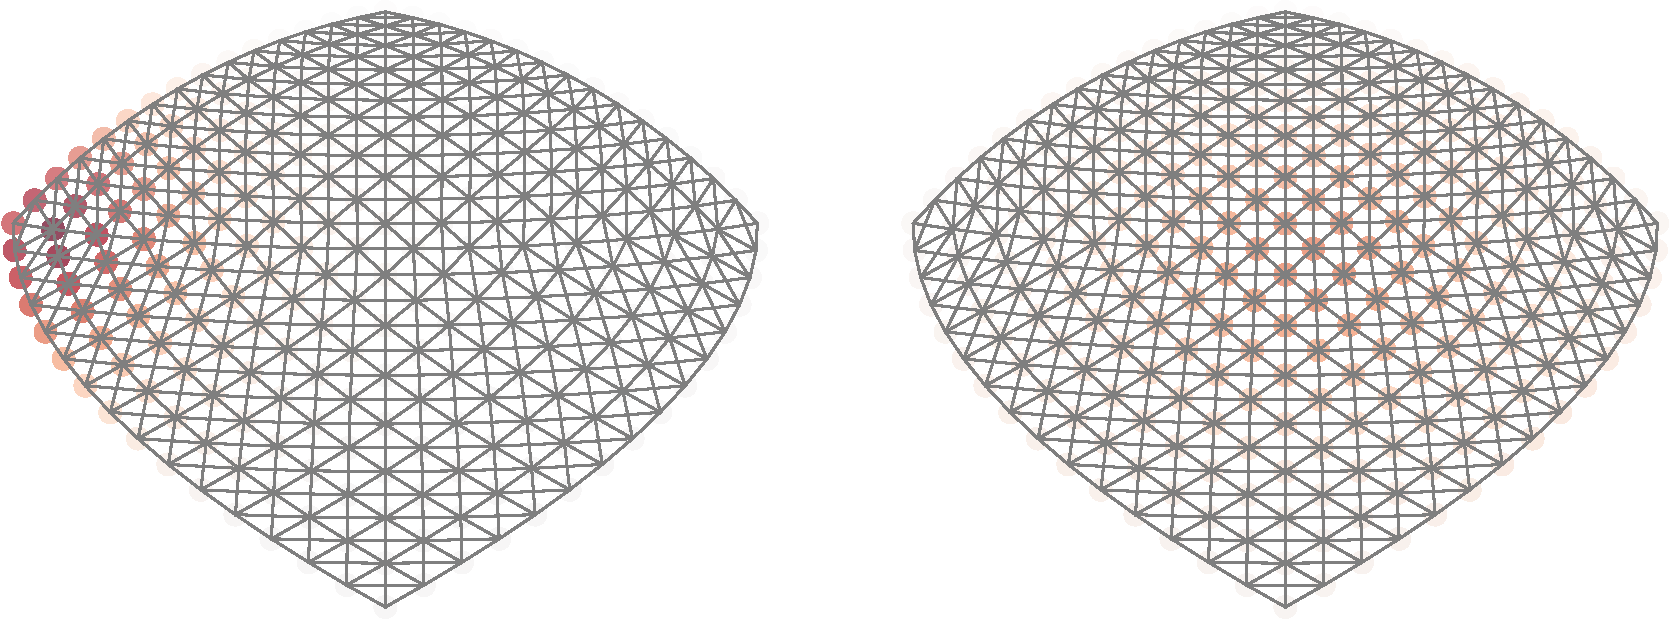
\includegraphics[width=\linewidth]{border_effects}
	\caption{Convolution kernel (also called filter) localized in the center and left corner of a graph built from $1/12^\text{th}$ of the sphere at $N_{side} = 16$.
		A filter $h$ is localized on a pixel $i$ as $\T_i h = h(\L) \b \delta_i$ (see \secref{graph_convolution}, equation~\eqnref{graph_convolution_spatial}).
	The filter is not isotropic anymore when localized on the corner as the graph representation of a manifold assumes reflective border conditions.}
	\label{fig:border_effects}
\end{figure}



Let us use the angular parametrization of the sphere $\mathcal{S}^2=\{\bf{x} | \|\bf{x}\|_2=1 \}$, in term of angles of zenith, $\theta\in [0,\pi ]$, and azimuth $\phi\in [0,2\pi[$.
\begin{equation}
\Phi(\theta, \phi) = (\sin \theta \cos \phi, \sin \theta \sin \phi, \cos \theta )
\end{equation}
Let $\mathcal(C)^\infty(\mathcal{S}^2)$ denote the class of infinitely differentiable functions $\mathcal{S}^2\rightarrow \mathbb{R}$. Using the agnular parametrization of the sphere, the Laplace-Beltrami for a function $f\in \mathcal(C)^\infty(\mathcal{S}^2)$ is given by:
\begin{equation}
\nabla_{\mathcal{S}^2} f = \frac{1}{\sin \theta } \frac{\partial}{\partial \theta} \left(\sin \theta  \frac{\partial f}{\partial \theta} + \frac{1}{\sin^2 \theta} \frac{\partial^2f}{\partial \phi^2} \right)
\end{equation}

% \begin{equation}
% \Lg \g{f}[i] := \frac{1}{n} \left( \g{f}[i]\sum_{j=1}^n k(x_i,x_j) -\sum_{j=1}^n \g{f}[j] k(x_i,x_j)\right)
% \end{equation}

For convergence we also need an extension operator:

% It is a generalization of the graph Laplacian operator that apply on a function $\p{f}:\M \rightarrow \Rbb $:
% \begin{equation}
% \Lp \p{f}(y) := \frac{1}{n} \left( \p{f}(y)\sum_{j=1}^n k(y,x_j)-\sum_{j=1}^n \p{f}(x_j)k(y,x_j) \right)
% \end{equation}


% $f\in \mathcal(C)^\infty(\mathcal{S}^2)$ and for a fixed point p \in M,
% after appropriate scaling the operator Lt
% n converges to the true Laplace–Beltrami operator on the manifold.



% Let us now focus on the convergence proofs. We consider a $k$-dimensional compact smooth manifold $\M$ embedded in $\Rbb^T$. The gradient of a $\mathcal{C}^1(\M)$ function $f$ evaluated in $\b{x}$ is given by $\grad_\M f(\b{x})$. It is a vector pointing in the direction of the fastest ascent of $f$. Note that the gradient evaluated in $\b{x}$ lives in the tangent space of the point $\b{x}$: $T_{\M}(\b{x}) \in \Rbb^k$. For convenience, we define the linear operator $\grad_{\G,v_i}$ to be the gradient vector at node $v_i$:
% \begin{equation}
% \left(\grad_{\G,v_i} \g{x}\right)[n] =
% \frac{\partial x}{\partial e_{in}} 
% = \sqrt{\Wg[i,n]} \left( \g{x}[n]-\g{x}[i] \right).
% \end{equation}
% Given a set of $N$ points $\{\b{x}_i\}_{i=1\dots N}$, we associate a complete weighted graph where each $\b{x}_i$ is associated to the vertex $v_i$ and we define the edges’ weights to be:
% \begin{equation} \label{eq:full_graph_gaussian_weight}
% \Weightf(v_i,v_n) = \Wg[i,n] = e^{\frac{\norm{\b{x}_i- \b{x}_n}_2^2}{4 t}},
% \end{equation}
% where $t$ is a positive constant depending on $N$. Using this special weight function, Belkin and Niogi have shown that the graph Laplacian converges to the Laplace-Beltrami operator of the manifold $\M$.
% \begin{theorem}[Theorem 3.1 of~\cite{belkin2005towards}, Laplacian convergence] \label{theo:laplacian_convergence_belkin}
% Let data points $\bf{x}_1,\dots, \b{x}_N$ be sampled from a uniform distribution on a manifold $\mathcal{M} \subset \Rbb^T$. Using the weight function \eqref{eq:full_graph_gaussian_weight}, define a sequence $t_N=N^{-\frac{1}{k+2+\alpha}}$, where $\alpha>0$ and let $f\in \mathcal{C}^\infty(\M)$, then the following holds:
% \begin{equation}
% \lim_{N \rightarrow \infty} \frac{1}{t_N(4\pi t_N)^{\frac{k}{2}}} (\Lg \b{f})[i] = \frac{1}{\vol (\M)} (\Lm f)(\b{x}_i)
% \end{equation}
% where the limit is taken in probability and $\vol(\M)$ is the volume of the manifold with respect to the canonical measure.
% \end{theorem}



The first 16 eigenvectors $[\b u_1, \ldots, \b u_{16}]$ of the graph Laplacian $\L$, forming the lower part of the graph Fourier basis $\U$, are shown in \figref{graph_harmonics}.
Let us further observe the spectral properties of our constructed spherical graph laplacian $\L$.
Its eigenvalues, shown in \figref{graph_eigenvalues}, are clearly organized in frequency groups of $2\ell + 1$ orders for each degree $\ell$.
We remind the reader that the amplitude of the Laplacian eigenvalue is proportional to the sum of the variations of its associated eigenvector. Furthermore, all spherical harmonics with the same order $\ell$ have the same variation. Hence, the fact that the Laplacian eigenvalues are grouped in blocks of size $2\ell + 1$ is a hint that the graph eigenvectors approximate the spherical harmonics.
In order to push the comparison one step further, we show the correspondence between the subspaces spanned by the graph Fourier modes and the spherical harmonics in \figref{subspace_harmonics_eigenvectors}.
%The block-diagonal structure of the matrix, as opposed to diagonal, results the fact that the phase of the graph eigenvector is not aligned with the one of the spherical harmonics.

\begin{figure}[t!]
	\centering
	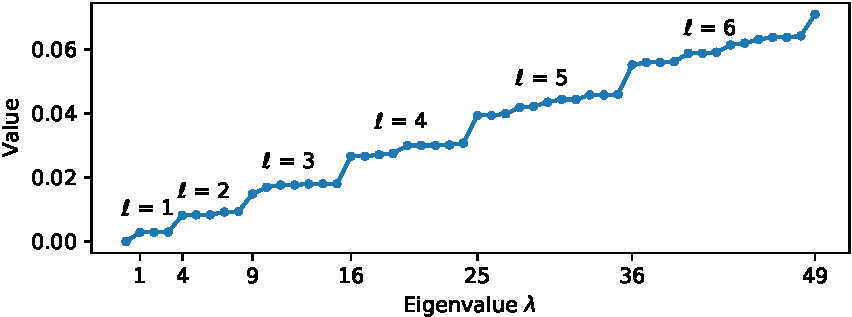
\includegraphics[width=\linewidth]{graph_eigenvalues}
	\caption{The eigenvalues $\bLambda$ of the graph Laplacian $\L = \U \bLambda \U\trans$, which corresponds to squared frequencies, are clearly organized in groups. Each group corresponds to a degree $\ell$ of the spherical harmonics. Each degree has $2\ell + 1$ orders. 
	See also \figref{graph_harmonics}.
	}
	\label{fig:graph_eigenvalues}
\end{figure}

\begin{figure}[t!]
	\centering
	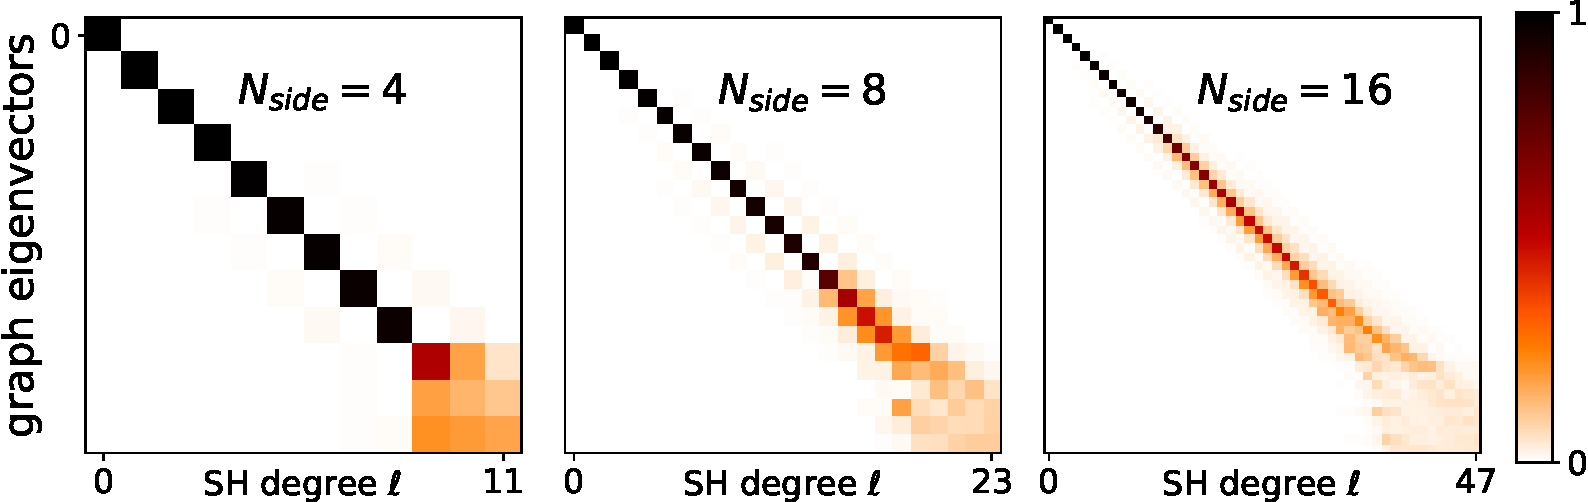
\includegraphics[width=\linewidth]{subspace_harmonics_eigenvectors_v2}
	\caption{Correspondence between the subspaces spanned by the graph Fourier modes and the spherical harmonics.
		The correspondance is computed in two steps. (i) We compute the PSD of each graph eigenvector.
		(ii) As, for each harmonic index $\ell$, there is $2\ell+1$ spherical harmonics, we sum the contribution of the corresponding $2\ell+1$ graph eigenvectors.
		% No real convergence with increasing Nside.
		% Row $j$ is the sum of the (normalized) power spectral densities (PSDs), computed by the SHT, of the $2j+1$ graph Fourier modes $\b u_i$ identified with degree $j$.
		% (\figref{graph_eigenvalues} shows how Fourier modes can be identified to spherical degrees.)
		% The PSD is computed for degrees $\ell=0$ to $\ell = 3 N_{side} -1$.
		% Pixel $k$ in row $j$ measures the energy in frequency band $k$ of the graph Fourier modes identified to be part of band $j$.
		The matrix should ideally be the identity.
		While not the case, the plot shows how the subspaces agree: the subspaces spanned by the Fourier modes correspond to those spanned by the spherical harmonics in the low frequencies, while the Fourier modes leak towards adjacent frequency bands in the high frequencies.
		While there is a systematic error, the Fourier modes agree at higher frequencies as $N_{side}$ increases.}
		\label{fig:subspace_harmonics_eigenvectors}
\end{figure}

While these indications show that the constructed graph Fourier basis approximates well the spherical harmonics, one should not forget that the small irregularities in the sampling (non-constant number of neighboring pixels and varying distance between pixels, see \figref{healpix_graph_4}) have an important effect on the graph Fourier modes.
First, we believe that they are responsible for energy leaking across frequency bands in \figref{subspace_harmonics_eigenvectors}.
Second, as the resolution is increased with $N_{side} \rightarrow \infty$ and $N_{pix} \rightarrow \infty$, we are still unsure if the eigenvectors would converge towards the spherical harmonics.
% We believe that it might be the case for a different construction of the graph (fully connected) and that a proof could be built on top of the work of~\cite{belkin2007convergence}. That is, however, out of the scope of this contribution.
The theoretical study of those phenomenons is left as future work.
Third, counter-intuitively, some eigenvectors will be localized~\citep{perraudin2018global}, i.e., they will span a small part of the sphere.
Those discrepancies result in a convolution operation that is not exactly equivariant to rotation.
Nevertheless, our experiments suggest that these downsides do not have an important effect on the convolution nor hinder the performance of the NN.


\todo{new results from Martino: becomes better in BN setting, currently under study}

\todo{we have less rich operations (compared to the most general linear equivariant map) by restricting our filters to be radial, but does it matter in practice?}
\todo{isotropic filters provide invariance to the third rotation}

\section{Experiments}

\todo{the cosmo experiment}

\todo{maybe mention some preliminary results on SHREC-17: we could say performance are so far mostly similar (while being invariant to the third rotation), still under study}

\section{Conclusion}  % & perspective

\todo{Generalization vs specialization: most general is to assume no symmetries (fully connected NN).
NNs can be specialized by adding some equivariance and invariance to symmetry groups such as translation, rotation, flip, etc.
More specialized NNs are more limited in the class of functions they can approximate, but requires less samples.
Again, use the right symmetries.}

\todo{As equivariance is not the Graal either. We expect the desired amount of equivariance to depend on the data and task. As usual, practitioners should adopt a NN architecture that exploit the symmetries of their problem. Cite paper with difference operators that is not equivariant but performs better than Cohen.}

\todo{future directions: equivalence / convergence to spherical harmonics, other tasks, comparison with other spherical CNNs, graph CNNs (especially those for manifolds), boundary conditions on partial sphere}

\textbf{Long term vision.}

We hope to establish graphs as a generic support for processing and learning over known and unknown manifolds.
\todo{Applications are plenty:
known manifolds (1D, 2D, 3D Euclidean spaces, circle, sphere)
% Minkowski spacetime
unknown manifolds (shapes, point clouds, feature sets)
}
\todo{
* known manifolds: grid, sphere, spacetime (a pseudo-Riemannian 4-manifold), surfaces defined by NURBS, anything else?
* unknown manifolds: meshes (human body), point clouds => what are the symmetries? local isometry
* non-manifold: all networks (brain, social, transportation, telecom, etc.) and relations (author-papers, user-products)
}

\todo{Similar goal: graph CNNs for group equivariant convolution.}

The vision is to push the use of graphs as the support for computation on manifolds. The advantages of graphs are to relax constraints on the sampling (e.g., allow an irregular or partial sampling), and be computationally more efficient (while being exact w.r.t. the continuous case).
Part of a broader research effort to explore the use of GSP to solve continuous problems.

\subsubsection*{Acknowledgments}

\todo{Pierre, Cardoso, Tomek?}

\bibliography{refs}
\bibliographystyle{iclr2019}

\end{document}
